
%----------------------------------------------------------------------------------------
%	PACKAGES AND OTHER DOCUMENT CONFIGURATIONS
%----------------------------------------------------------------------------------------

\documentclass[12pt]{article}
\usepackage[english]{babel}
\usepackage[utf8x]{inputenc}
\usepackage{amsmath}
\usepackage{graphicx}
\usepackage[colorinlistoftodos]{todonotes}
\addto\captionsbrazilian{}

\begin{document}

\begin{titlepage}

\newcommand{\HRule}{\rule{\linewidth}{0.5mm}} % Defines a new command for the horizontal lines, change thickness here

\center % Center everything on the page
 
%----------------------------------------------------------------------------------------
%	HEADING SECTIONS
%----------------------------------------------------------------------------------------

\textsc{\normalsize UNIVERSIDADE DE BRASÍLIA}\\[1.0cm] % Name of your university/college
\textsc{\Large Organização e Arquitetura de Computadores}\\[0.2cm] % Major heading such as course name
\textsc{\large  Turma B - Laboratório 01}\\[0.2cm] % Minor heading such as course title

%----------------------------------------------------------------------------------------
%	TITLE SECTION
%----------------------------------------------------------------------------------------

\HRule \\[0.4cm]
{ \huge \bfseries \LARGE{DESENVOLVIMENTO DE APLICAÇÕES EM ASSEMBLY MIPS} \\ [1.0cm]
\emph{\large{Agenda de Contatos Eletrônica}}
}\\[0.4cm] % Title of your document
\HRule \\[1.0cm]
 
%----------------------------------------------------------------------------------------
%	AUTHOR SECTION
%----------------------------------------------------------------------------------------

%\begin{minipage}{0.4\textwidth}
%\begin{flushleft} \large
%\emph{Alunos:}\\
%André Luiz Silveira - 12/0126648 \\Lucas %\textsc{Smith} % %Your name
%Rafael 
%\end{flushleft}
%\end{minipage}
%~

\begin{minipage}{0.4\textwidth}
\begin{flushright} \large
\emph{Professor:} \\
Flávio \textsc{Vidal} % Supervisor's Name
\end{flushright}
\end{minipage}\\[2cm]

% If you don't want a supervisor, uncomment the two lines below and remove the section above
\flushleft \Large \emph{Alunos:}\\ 
Lucas Villela de Souza Lacerda (Líder) - 12/0126648\\ 
Victor Fabro Neri - 12/0153939 \\ % Your name

%----------------------------------------------------------------------------------------
%	DATE SECTION
%----------------------------------------------------------------------------------------

\center {\large 23 de Abril, 2017}\\[2cm] % Date, change the \today to a set date if you want to be precise

%----------------------------------------------------------------------------------------
%	LOGO SECTION
%----------------------------------------------------------------------------------------


\includegraphics[scale = 0.3]{logo1.jpg}\\[1cm] % Include a department/university logo - this will require the graphicx package
 
%---------------------------------------------------------------------------------------- FOLHA DE ROSTO

\begin{titlepage}
\vfill
\begin{center} 
{\large Lucas Villela \\  [0.1cm]
Victor Neri } \\[5cm] 
{\Huge DESENVOLVIMENTO DE APLICAÇÕES EM ASSEMBLY MIPS}\\[1cm]
\hspace{.45\textwidth} % posicionando a minipage
\begin{minipage}{.5\textwidth}
Agenda de Contatos Eletrônica
\end{minipage}
\vfill
23 de Abril, 2017
\end{center}
\end{titlepage}

%-------------------------------------------------------------------
\vfill % Fill the rest of the page with whitespace

\end{titlepage}

\section{Objetivos}
\textit{\paragraph{}
	Permitir que o aluno(a) se familiarize com a linguagem Assembly MIPS e metodologias de aplicações eficientes e otimizadas. Esta atividade tem como intuito formar espírito crítico de avaliação a respeito do desempenho real provido pelo sistema computacional, proporcionando assim melhorias na compreensão do funcionamento destes tipos de sistemas.
	\paragraph{}
	O projeto desta disciplina é uma atividade planejada de forma a complementar e reforçar o conteúdo programárico da disciplina Organização e Arquitetura de Computadores. Espera-se qua nas atividades de projeto os alunos desenvolvam sua capacidade de observação, análise e compreensão das metodologias de OAC.
	\paragraph{}	
	Desta forma cabe ao aluno(a) ou grupo, partindo da premissa que possui os requisitos para o curso, juntamente com o conteúdo adquirido nas aulas teóricas, desenvolver todas as etapas da implementação solicitada.}\\[1.0cm]

\section{Introdução}

    \paragraph{}
   	Para controlar o hardware de um computador é preciso falar sua linguagem. As palavras da linguagem de um computador são chamadas instruções e seu vocabulário é denominado conjunto de instruções.
   	\paragraph{}                    
	Em uma análise superficial, pode-se pensar que as linguagens dos computadores são tão diversificadas quanto as linguagens humanas, mas, na realidade, as linguagens de computador são muito semehlante entre si e mais parecidas com dialetos regionais do que idiomas independentes. Assim, ao aprender uma das linguagens, aprender as outras se torna fácil. Essa semelhança ocorre porque todos os computadores são construídos a partir de tecnologias de hardware baseadas em princípios básicos semelhantes e porque existem algumas operações básicas que todos os computadores precisam oferecer. Além do mais, os projetistas de computadores possuem um objetivo comum: Encontrar ma linguagem que facilite o projeto do hardware e do compilador enquanto maximiza o desempenho e minimiza o custo. 
	\paragraph{}
	O conjunto de instruções escolhido vem da MIPS Technology, que é um exemplo elegante dos conjuntos de instruções criados desde a década de 1980.
	
\subsection{Operandos do hardware do computador}
    \paragraph{}
    Diferente de programas em linguagens de alto nível, os operandos das instruções aritméticas são restritos, precisam ser de um grupo limitado de locais especiais, embutidos dirteamente no hardware, chamados registradores. Os registradores são primitivas usadas no projeto do hardware que também são visíveis ao programador quando o computador é completado. Otamanho de um registrador na arquitetura MIPS é de 32 bits; os grupos de 32 bits ocorrem com tanta frequência que recebem o nome de palavra(word) na arquitetura MIPS.
    \paragraph{}
    Uma diferença importante entre as variáveis de uma linguagem de programação e os registradores é o número limitado destes, normalmente 32 ou 64 nos computadores mais modernos.
    \paragraph{}
    O motivo para o limite de 32 registradores é a fidelidade a um dos princípios de projeto básicos da tecnologia de hardware que diz:
\textit{\paragraph{}Menor significa mais rápido.}
    \paragraph{}
    Uma quantidade muito grande de registradores pode aumentar o tempo do ciclo do clock simplesmente porque os sinais eletrônicos levam mais tempo quando precisam atravessar uma distancia maior.
    \paragraph{}
    Obviamente sabemos quepremissas como "Menor significa mais rápido" não são absolutas. 31 registradores podem não ser mais rápidos que 32. Mesmo assim, a verdade por trás dessas observações faz com que os prjetistas de computadores as levem a sério . Sendo assim, o projetista precisa equilibrar o desejo dos programas por mais registradores como o desejo do projetista de manter o ciclo de clock rápido.Outro motivo para não usar mais de 32 é o número de bits que seria necessário no formato das instruções.
    \paragraph{}
    Embora pudéssemos simplesmente escrever instruções usando números para os registradores, de 0 a 31, a convenção do MIPS é usar nomes com um sinal de cifrão seguido por dois caracteres para representar um registrador.usaremos $s0, $s1... para os registradores que correspondem às variáveis dos programas em C e Java, e $t0, $t1... para os registradores temporários necessários para compilar o programa nas instruções MIPS.
    
\begin{figure}[h!]
    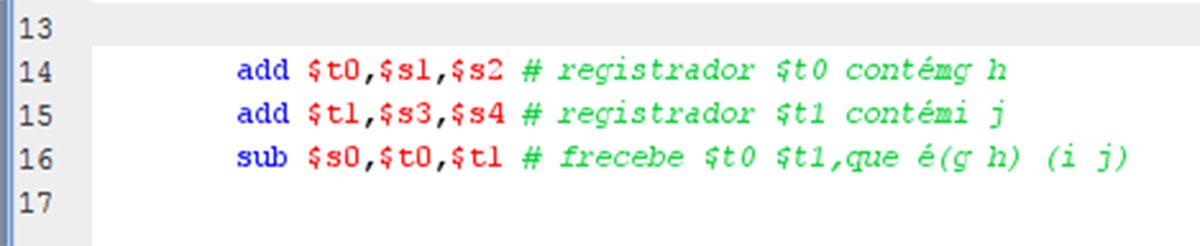
\includegraphics[width=\linewidth]{exemplo1.jpg}
    \caption{Exemplo de código que implementa a expressão f=(g+h)−(i+j).}
    \label{fig:codigo_soma}
\end{figure}

\subsection{Operando em memória}
    \paragraph{}
    Além de elementos de dados isolados, as linguagens de programação possuem também estruturas de dados mais complexas. Essa estruturas de dados complexas podem conter muito mais elementos de dados do que a quantidade de registradores em um computador. O processador só mantém uma pequena quantidade de dados nos registradores , mas a memória do computador contém milhões de elementos  de dados. Logo, as estruturas de dados (arrays e estruturas) são mantidas na memória.
    \paragraph{}
    Conforme explicado, as operações aritméticas só ocorrem nos registradores. Assim, o MIPS precisa incluir instruções que transferem dados entre a memória e os registradoresEssas instruções são denominadas instruções de transferência de dados. Para acessar uma palavra na memória, a instrução precisa fornecer o endereço de memória. A memória é apenas uma sequência grande e unidimensional,com o endereço atuando como índice para esse array, começando de 0.Por exemplo, na figura abaixo, o endereço do terceiro elemento de dados é 2 e o valor de Memória[2] é 10.

\begin{figure}[h!]
    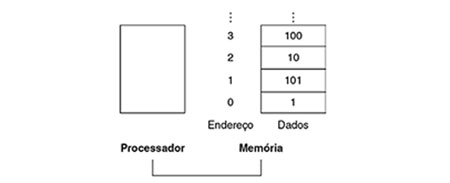
\includegraphics[width=\linewidth]{memoria.jpg}
    \caption{Endereços e conteúdo da memória.}
    \label{fig:memoria}
\end{figure}

    \paragraph{}
    A instrução de transferência de dados que copia dados da memória para um registrador tradicionalmente é chamada de load. O formato da instrução load é o nome da operação seguido pelo registrador a ser carregado, depois uma constante e o registrador usado para acessar a memória. A soma da parte constante da instrução com o conteúdo do segundo registrador forma o endereço da memória. O nome MIPS real para essa instrução é lw, significando load word (carregar palavra).
\subsection{Operandos Imediatos}
    \paragraph{}
    Muitas vezes, um programa usará uma constante em uma operação – por exemplo, ao incrementar um índice a fim de apontar para o próximo elemento de um array. Na verdade,mais da metade das instruções aritméticas do MIPS possuem uma constante como operando quando executam os benchmarks SPEC2006. Usando apenas as instruções vistas até aqui, teríamos de ler uma constante da memóriapara utilizá-la. (As constantes teriam de ser colocadas na memória quando o programa fosse carregado.) Por exemplo, para somar a constante 4 ao registrador s3, poderíamos usar o código
    
\begin{figure}[h!]
    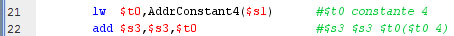
\includegraphics[width=\linewidth]{exemplo2.jpg}
    \caption{Carregando um valor sem instruções tipo I.}
    \label{fig:memoria}
\end{figure}

    supondo que AddrConstant4 seja o endereço de memória da constante 4.
    \paragraph{}
    Uma alternativa que evita a instrução load é oferecer versões das instruções aritméticas em que o operando seja uma constante. Essa instrução add rápida, com uma constante no lugar do operando, é chamada add imediato, ou addi. Para somar 4 ao registrador s3, simplesmente escrevemos
    
\begin{figure}[h!]
    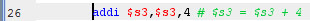
\includegraphics[width=\linewidth]{exemplo3.jpg}
    \caption{Exemplo de opedação com imediatos.}
    \label{fig:memoria}
\end{figure}

    \paragraph{}
    As instruções imediatas ilustram mais um dos princípios do projeto de hardware, que diz:
\textit{\paragraph{}Agilize os casos mais comuns.}
    \paragraph{}
    Os operandos constantes ocorrem com frequência e, incluindo constantes dentro das instruções aritméticas, as operações são muito mais rápidas e usam menos energia do que se as constantes fossem lidas da memória.
    \paragraph{}
    A constante zero tem outro emprego, que é simplificar o conjunto de instruções por oferecer variações utéis. Por exemplo, a operação mova é apenas uma instrução de soma na qual cada operando é zero. Portanto, o MIPS dedica o registrador zero para ter o valor zero. (Que no caso, é o registrador zero.)
    \paragraph{}
    A imagem abaixo é um resumo dos aspectos básicos da arquitetura MIPS, contendo as algumas das instruções mais usadas para programas básicos 
    \paragraph{}
    .
    \paragraph{}
    .
\begin{figure}[h!]
    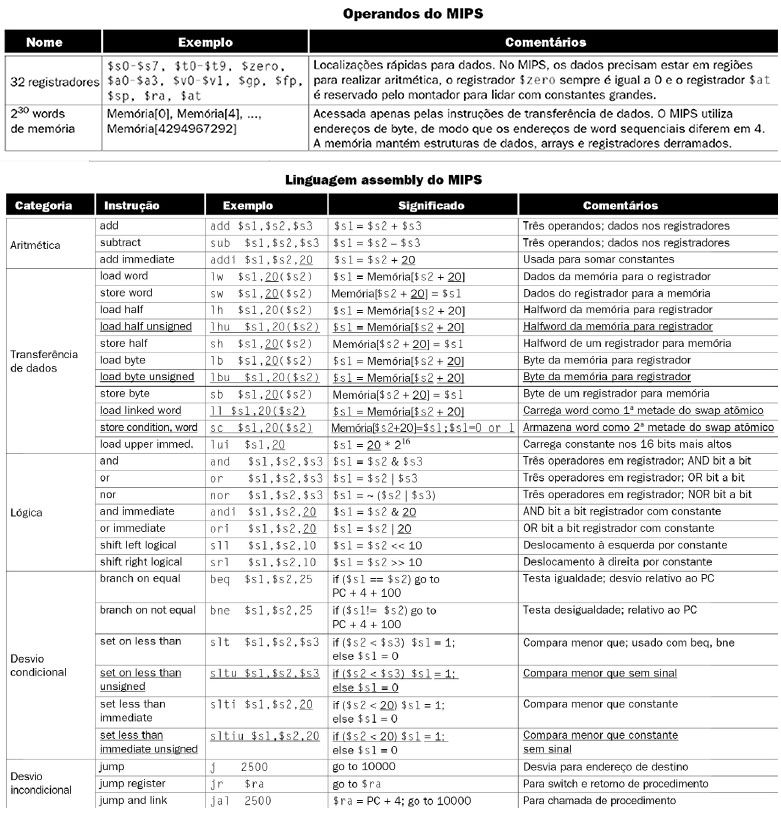
\includegraphics[width=\linewidth]{tudomips.jpg}
    \caption{Introdução à arquitetura MIPS.}
    \label{fig:MIPS_overview}
\end{figure}

    \paragraph{}
    .
     \paragraph{}
    .
    \paragraph{}
    .
    \paragraph{}
    .

\section{Materiais e Métodos}
\label{sec:examples}
    \paragraph{}
    Para a realização do experimento foi utilizado apenas um computador e o software de simulação MARS. Tal simulador permite que sejam criados programas em linguagem Assembly MIPS.
	\paragraph{}
	Após aberto o MARS, foi criado um novo arquivo e salvo com extensão .asm. Em seguida, foi criada uma diretiva .data (os itens subsequentes são armazenador em um segmento Data no próximo endereço disponível).
	\paragraph{}
	Dentro dela, foram criados rótulos com diretivas próprias. As diretorias utilizadas foram: .asciiz (armazena uma string em um segmento Data e adiciona um terminador nulo, onde o que vai ser armazenado deve estar dentro de aspas ""); .space (reversa o espaço determinado de bytes no segmento Data).
	
\begin{figure}[h!]
    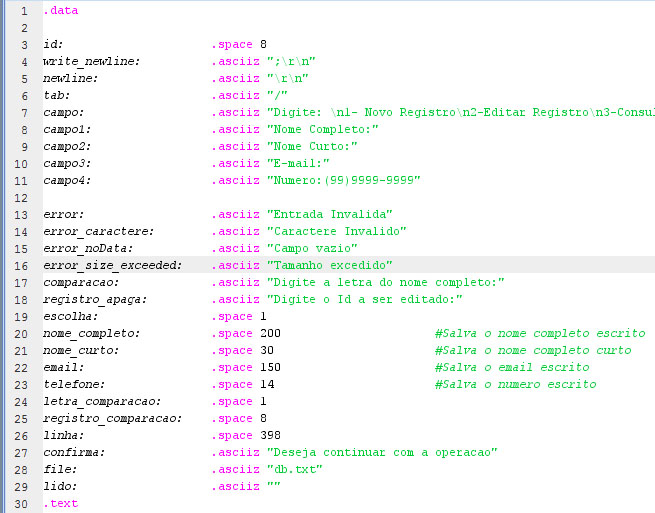
\includegraphics[width=\linewidth]{dados.jpg}
    \caption{Area de dados.}
    \label{fig:areadedados}
\end{figure}

    \paragraph{}
    Ao analisar as linhas 2 e 3, é possível perceber que rótulos tab e linha foram definidos como strings e possuem dentro de si "contrabarra t" e "contrabarra n"; onde "contrabarra t" e "contrabarra n" não aparece nada, dando apenas um tab na saída e pulando uma linha, respectivamente. 
	\paragraph{}
	Depois, foi criada a diretiva .text (os subsequentes itens são instruções armazenadas em um segmento Text no próximo endereço disponível).
	\paragraph{}
	O código simula uma agenda de contatos simples, similar às agendas de contatos em celulares. Para tal simulação, foram usados vários recursos que o MARS dispõe, tais como o console de I/O, as syscalls de uso de interface gráfica e syscalls de manipulação em arquivos. 
	\paragraph{}
	A agenda possui cinco funções básicas: criar um novo contato, editar um contato existente, consultar informações de um contato, visualisar uma lista de contatos e apagar um contato. Os contatos e suas informações são salvos em um banco de dados, simulado por um arquivo de texto simples. 
	
\begin{figure}[h!]
    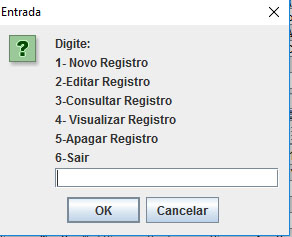
\includegraphics[width=\linewidth]{menu.jpg}
    \caption{Menu principal.}
    \label{fig:menuprincipal}
\end{figure}	
	
	\paragraph{}
	Na primeira parte do código, a instrução "jal" pula para a o procedimento que implementa o menu principal.
	\paragraph{}
	O menu (e boa parte do programa) é implementado usando as syscalls de número 50 a 55, onde é possivel usar caixas de diálogo tanto para colher dados quanto para mostrar mensagens de erro. Na função do menu podemos ver os parâmetros da syscall 54 sendo preparados antes da chamada do sistema. Dopois da primeira syscall, o menu de escolha aparece pedindo o numero da operação desejada, e o que foi digitado é salvo no buffer chamado "escolha".
	\paragraph{}
	Na segunda parte da função, o código verifica o registrado a1, que salva o status da operação anterior e, se houver algum parâmetro que indique erro, o código desvia para a função de erro adequada, mostrando uma mensagem e volta para o menu para que a escolha seja digitada corretamente.
	\paragraph{}
	Já com os dados de escolha corretos, o código verifica qual foi a escolha feita e desvia para o prcedimento adequado. Se for digitado "1", cria um novo registro, "2" edita um registro, "3" consulta um registro, "4" visualiza os registros, "5" apaga um registro e "6" encerra o programa.
\subsection{Criando novo contato}
    \paragraph{}
    Esta função coleta 4 strings de dados:
    \begin{itemize}
    \item Nome completo
    \item Nome curto
    \item E-mail
    \item Telefone
    \end{itemize}
    
    \paragraph{}
    O algoritmo e funcionamento desta opção é descrito agora. Primeiramente, ao digitar "1" no menu, o código abre o arquivo para leitura, lê o arquivo para pegar o último número ID e somar 1, e fecha o arquiv novamente.
    \paragraph{}
    Em seguida, é aberto o arquivo no modo de escrita, o usuário digita o nome completo na caixa que aparece, o código armazena o dado em memória. O mesmo é repetido para o campo "Nome curto", "E-mail" e "Telefone".
    \paragraph{}
    Depois, vamos para a função de contagem de letras, onde será contado o número de letras de cada um desses campos. Após a última letra de "Nome completo", "Nome curto" e "E-mail" é adicionado uma barra ("/"), que foi escolhido como caractere de delimitação de campo dentro de um mesmo registro. Após o campo "telefone", que é o último campo do registro, é colocado um ponto-e-vírgula (";"), caractere escolhido para delimitação de registro. 
    \paragraph{}
    Isso tudo é feito ma memória, por conveniência. Em seguida vamos para a função "writefile" para escrever o registro no arquivo. Os campos são escritos no arquivo nessa ordem: "ID", "Nome completo", "Nome curto", "E-mail", "Telefone".
    \paragraph{}
    Enfim o código fecha o arquivo e retorna ao menu principal.
    
\subsection{Editando um contato}
    \paragraph{}
    Primeiro, depois de digitar "2" no menu, o arquivo é abert para leitura com "openfile", depois é lido inteiro e gravado inteiro na memória (buffer de nome "lido"). Uma vez copiado o arquivo para a memória, abrimos o arquivo para escrita com a flag "1". Isso serve apenas para apagar todo o arquivo. Em seguida o arquivo é fechado.
    \paragraph{}
    Após essa parte, é solicita o ID do registro a se editado. Esse número é salvo na memória e será usado para buscar na memória a linha do registro a ser editado. 
    \paragraph{}
    A busca na memória se inicia percorrendo o buffer "lido", que contém a cópia do arquivo, até o final da primeira linha. Essa linha é salva no buffer "linha". Daí, comparamos os 8 primeiros dígitos de "linha" (ou seja, o ID do registro) e comparamos com o ID salvo. Se forem diferentes, essa linha é escrita no arquivo. Se for igual ele pula para o procedimento de "novo registro", editando assim o registro desejado (há uma ondicional para não somar +1 no ID quando se está editando).
    \paragraph{}
    Depois de editado e reescrito o arquivo todo com o processo acima, depois da ultima linha é fechado o programa.
\subsection{Consultar}
    \paragraph{}
    Depois de digitar "3" no menu, o arquivo é abert para leitura com "openfile", depois é lido inteiro e gravado inteiro na memória (buffer de nome "lido"). Uma vez copiado o arquivo para a memória, o arquivo é fechado e aparece uma caixa pedindo a primeira letra do nome. Essa letra é salva para futura comparação.
    \paragraph{}
    Após isso, o programa percorre "lido" e grava a primeira linha em "linha". Depois o programa compara a letra anteriormente salva com o nono caractere contido em "linha" (os 8 primeiros são o ID, o nono é a primeira letra do nome). Se forem iguais, o registro é impresso no console I/O do MARS, e depois retorna ao menu principal. Se for diferente, o código avança para a próxima linha da cópia do arquivo e repete o algoritmo aqui descrito até a ultima linha da cópia do arquivo, voltando para o menu principal.
\subsection{Visualizar Registros}
    \paragraph{}
    Essa opção mostra no console Todos os registros. Depois de digitar "4" no menu, o código abre o arquivo para leitura, lê o arquivo completo e faz uma cópia em "lido", e fecha o arquivo.
    Após isso, o programa percorre lido e grava a primeira linha em "linha". Depois é usada a syscall 4 para printar essa linha no console. Depois zeramos o buffer "linha", percorremos a segunda linha de "lido" e a grvamos em "linha", repetindo o processo sucessivas vezes até ser impressa a última linha. Depois retornamos ao menu principal.
\subsection{Apagar um contato}
    \paragraph{}
    Essa função age de modo semelhante à função de editar. Mas, em vez de pedir os novos dados (se o ID for o desejado) ele apenas pula uma linha, excluindo o registro de ID salvo pelo usuário. Após a escrita no arquivo da última linha, o programa é encerrado. 
    
\subsection{Limitações do programa}
    \paragraph{}
    O programa tem algumas limitações. Nas opções de edição (Editar contato e Apagar), por exemplo, após a edição ser cocluída, o programa é encerrado. O comportamendo desejado seria que o programa retornasse ao menu principal. Porém, quando adicionamos a parte de código que volta para o menu principal, as opções de visualização e consulta deixam de funcionar. Visto que essa falha nos estava consumindo muito tempo, optamos por fechar o programa antes que as outras opções parassem de funcionar pois era necessário um código com todas as opções funcionais e sem prejuízo no banco de dados para obter do Instruction Statics dados confiáveis.
    \paragraph{}
    Outro problema resolvido de modo alternativo foi o botão "cancelar". Quando se usa um botão de cancelar é esperado que a operação seja realmente cancelada. Isso significa que tudo no arquivo que de algum modo foi alterado durante o código deveria ser "desalterado". Tentando evitar a implementação de uma função cancelar (por falta de tempo), o programa mostra uma caixa de confirmação da operação de Editar/Apagar e, uma vez que se aperta o "sim", as caixas de edição só somem quando algo válido é digitado e, durante uma edição, o botão cancelar retorna para a caixa de entrada de dados até que seja digitado algo válido.
    \paragraph{}
    E por fim, há um limite de registros que podem ser feitos (1000 registros), mas que pode ser alterado via código. Basta ir na função "readfile" (linha 134) e alterar o número salvo no registrador a2. Por padrão, o número que se encontra no código é 398000, onde 398 é o tamanho de caracteres máximos que ocupa uma linha. logo, 398(quantidade de registros=1000) =398000.
\section{resultados}
    \paragraph{}
    Ao compilar o código, utilizando a ferramenta Instruction Statistics fornecida pelo MARS, foi montada a tabela a seguir (dividida em duas) com as porcentagens de utilização das instruções utilizadas em cada procedimento, onde cada procedimento é uma opção do menu principal.
    \paragraph{}
        
\begin{table}[h!]
  \centering
  \caption{Parâmetros X Procedimentos.}
  \label{tab:table1}
  \begin{tabular}{c||c|c|c}
   
    Parâmetro & Procedimento 0 & Procedimento 1 & Procedimento 2 \\
    \hline
    ULA & 64 & 41 & 41\\
    \hline
    Jump & 5 & 14 & 14\\
    \hline
    Branch & 5 & 27 & 25\\
    \hline
    Memory & 0 & 18 & 19\\
    \hline
    Others & 27 & 1 & 1\\
  \end{tabular}
\end{table}


\begin{table}[h!]
  \centering
  \caption{Parâmetros X Procedimentos.}
  \label{tab:table2}
  \begin{tabular}{c||c|c|c}
   
    Parâmetro & Procedimento 3 & Procedimento 4 & Procedimento 5 \\
    \hline
    ULA & 41 & 41 & 41\\
    \hline
    Jump & 14 & 14 & 14\\
    \hline
    Branch & 26 & 26 & 25\\
    \hline
    Memory & 19 & 19 & 20\\
    \hline
    Others & 1 & 1 & 1\\
  \end{tabular}
\end{table}

    \paragraph{}
    O procedimento 0 é o pedaço de código que vai do início da execução do programa até aparecer a caixa do menu principal. O procedimento 1 é a criação de um contato. O procedimento 2 é a edição de um contato. O procedimento 3 é a consulta a contato. O procedimento 4 é a visualização da lista de contatos cadastrados> e finalmente, o procedimento 5 é apagar um contato. 
	\paragraph{}
	O valor das procentagens, embora muito parecidos nos procedimentos, faz bastante sentido uma vez que seus algoritmos são bastante similares entre siutilizam as mesmas funções no código para operar, mudando apenas alguns detalhes. Os procedimentos 2 e 5 derivações do procedimento 1, assim como acontece com os procedimentos 3 e 4.
	\paragraph{}
	Além disso a grande maioria das instruções são do tipo R, lw ou sw, o que explica a maior porcentagem estar associada à ULA. O programa faz uma quantidade considerável de testes, sendo o próprio menu principal implementado com branches, explicando assim a razão de a segunda maior pocentagem estar ligada aos Branches.
	\paragraph{}
	A aplicação faz bastante uso da memória. Ela é usada para exibir mensagens, guardar entradas do usuário, armazenar caracteres frequentemente utilizados (delimitadores de campo, newline, etc), armazena as strings das mesagens de erro e faz cópias do arquivo várias vezes. Por isso, a memória fica com a terceira maior porcentagem de uso. E por ultimo ficam os Jumps, que são mais frequentes no final de procedimentos visto que o programa é estruturado em funções. Porém os jumps não são tão usados quanto os Branches e a Memória.
\section{Discussões e conclusões}
\subsection{Desempenho}
    \paragraph{}
    Geralmente, a melhoria de um único aspecto não aumenta o desempenho geral de forma considerável. Porém nesse caso, as porcentagens de uso de cada parâmetro são bem parecidas e ainda todos os procedimentos compartilham instruções e funções, pode-se afirmar que a melhoria do uso de algum dos parâmetros afetaria diretamente no desempenho geral, melhorando a velocidade de todos os outros procedimentos e, logo, do programa inteiro.
    \paragraph{}
    Outra método a se usar para a mehloria do desempenho do código é usar os princípios de projeto desde o começo do desenvolvimento. Um deles é: 
    \textit{\paragraph{}Agilizar o caso comum.}
    \paragraph{}
    Essa orientação simples faz lembrar que, em muitos casos, a frequência que um evento ocorre  pode ser muito mais alta do que outros eventos, logo, agilizar o caso mais comum é mais impactante no desempenho do que agilizar o caso mais raro.
    \paragraph{}
    Na maioria das vezes, em agendas de contatos comuns,  a consulta ao contato é o caso mais comum. Então uma hipotese para melhoria do desempenho seria agilizar a consulta aos registros. 
\subsection{Conclusões}
    \paragraph{}
    Tendo em mente novamente os objetivos deste primeiro laboratório, a criação desta aplicação foi essencial para o aprendizado da linguagem Assembly MIPS, que possui lógica e abstrações bem diferentes e menos intuitivas do que as linguagens de mais alto nível anteriormente estudadas.
    \paragraph{}
    E ainda, por mais que este código não esteja bem otimizado, desenvolvê-lo nos deu uma boa noção de como fazer melhor esse tipo de projeto. Tabém aprendemos bastante sobre o vocabulário do MIPS por usá-lo na prática.
    \paragraph{}
    Os aspectos teóricos também foram bastante abordados durante a execução do projeto, conjunto de instruções, registradores, memória, simulação de banco de dados simplificado, atingindo todos os requisitos básicos do projeto.

\section{Referências bibliográficas}
\begin{itemize}
\item PATTERSON, David A.; HENNESSY, John L. \textit{Organização e Projeto de Computadores - Interface hardware/software}. 4ª edição.
\end{itemize}

\end{document}
